\chapter{Einleitung}



\section{Test Driven Development}

Die testgetriebene Entwicklung (im englischen \textit{test-driven development} oder kurz TDD, wird auch \textit{test first development} genannt) ist ein Teil der agilen Softwareentwicklung und basiert darauf, dass die Tests vor dem Produktivcode geschrieben werden. Da Diese dabei eine zentrale Rolle spielen, geben wir zunächst einen Überblick über die unterschiedlichen Arten. Im Anschluss gehen wir detaillierter auf die testgetriebene Entwicklung ein.

\subsection{Arten von Tests}

Tests sollen einen bestimmten Teil des Programms auf seine Korrektheit überprüfen und dabei möglichst schnell und automatisiert ablaufen. Je nachdem wie umfangreich der getestete Bereich ist und welche Kenntnisse der Test/Entwickler von der inneren Umsetzung des Programms hat, kann man die Tests kategorisieren.

\paragraph{White- und Black-Box-Tests} Die gröbste Einteilung ist die Unterscheidung zwischen White- und Black-Box-Tests. Dabei wird nicht der Umfang des getesteten Bereichs berücksichtigt, sondern lediglich ob der Entwickler des Tests Kenntnisse über die Implementierung der zu testenden Funktionen hat.\\
Bei White-Box-Tests ist dies der Fall. Idealerweise, sollte der Entwickler der den Produktivcode geschrieben hat auch den dazugehörigen Test implementieren. Mit dieser Art von Test werden die inneren Strukturen eines Programms überprüft. Also zum Beispiel, dass eine Methode nicht mit Parametern aufgerufen werden kann, die Fehler verursachen könnten. Hierbei wird nur getestet ob das Programm fehlerfrei abläuft und nicht ob die einzelnen Methoden das gewünschte Verhalten aufweisen.

Im Gegensatz dazu stehen die Black-Box-Tests, deren Entwickler keinerlei Kenntnisse über die Umsetzung haben sollte. Ansonsten könnten beim Schreiben der Tests Dinge implizit als erfüllt angesehen werden, die allerdings getestet werden müssen. Dadurch wäre es möglich, dass bei nachträglichen Änderungen Fehler auftreten, ohne dass ein Test fehlschlägt.\\
Black-Box-Tests sollen verifizieren, dass das Programm die Spezifikationen des Kunden erfüllt.

Diese beiden Testarten ergänzen sich gegenseitig und es sollten immer sowohl White-Box, als auch Black-Box-Tests erstellt werden, um das Produkt zu überprüfen und robust gegen Fehler bei nachträgliche Änderungen zu machen.\\
Schematische Darstellungen dieser Testarten sieht man in \autoref{fig:White_Box_Test} und \autoref{fig:Black_Box_Test} auf den nächsten Seiten.

\paragraph{Unit-Tests} sind die kleinsten Einheiten unter den Tests. Sie sollen die einzelnen Methoden einer Klasse auf einen fehlerfreien Ablauf und ein korrektes Verhalten hin testen. Dadurch kann man im Verlauf der Entwicklung Änderungen am Programm vornehmen, ohne dass die Funktionalitäten der Module unbemerkt zerstört werden (insofern die Tests eine ausreichende Abdeckung erreichen).\\
Die einzelnen Tests sollten unabhängig voneinander und auch von den anderen Komponenten sein. Falls Verbindungen zwischen den Komponenten bestehen, sollten diese durch \textit{Mock}-Objekte entkoppelt werden. Diese erben von der entsprechenden Klasse und überschreiben deren Methoden auf eine geeignete Art. Zum Beispiel könnten sie einfach leer gelassen werden, was man als \textit{Stub} bezeichnet. Oder sie geben einen festen Wert zurück. \textit{Mock}-Klassen können selbst erstellt werden und sind meistens innere Klassen der Testklasse, allerdings gibt es auch \textit{Mock}-Frameworks, welche generisch \textit{Mocks} für beliebige Klassen oder Interfaces erzeugen können. Das Verhalten der Methoden eines Mocks, lässt sich mit diesen zur Laufzeit festlegen. Zum Beispiel dass ein fester Wert zurückgeliefert wird, oder eine Exception geworfen werden soll.\\ Beispiele sind \textit{JMock} für Java oder \textit{Moq} für C\#.\\
Außerdem sollten Unit-Tests sehr schnell ablaufen (im Millisekunden-Bereich), um nach jeder Änderung durchgeführt werden zu können, ohne die Entwicklung aufzuhalten.

Eine schematische Darstellung von Unit-Tests sieht man in \autoref{fig:Unit_Test}.

\paragraph{Integrationstests} Die nächsthöhere Stufe von Tests sind Integrationstests. Diese testen das Zusammenspiel mehrere Komponenten, eventuell auch mit Systemressourcen, auf ihre Korrektheit. Einen Unit-Test kann man zu einem Integrationstest machen, indem man die \textit{Mock}-Objekte durch die im Produktivbetrieb verwendet Klassen ersetzt und die Bedingungen entsprechend anpasst.

Integrationstests dürfen länger dauern als Unit-Tests, sollten dennoch schnell durchgeführt werden können.

Eine schematische Darstellung von Integrationstests sieht man in \autoref{fig:Integration_Test}.\\\\\\\\\\

\begin{figure}[h]
\centering
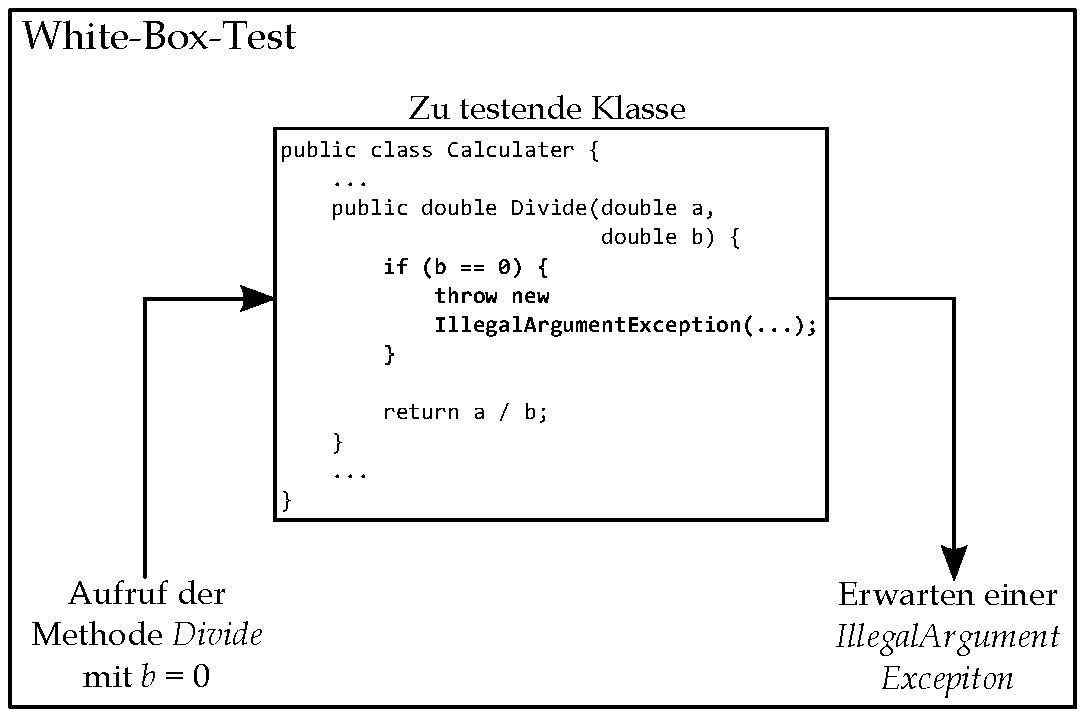
\includegraphics[width=0.8\linewidth]{./images/Kapitel_Einleitung/White_Box_Test.pdf}
\caption[Schematische Darstellung eines White-Box-Tests]{Schematische Darstellung eines White-Box-Tests\\Der Entwickler sollte sich gut mit dem zu testenden Code auskennen. Der Test verifiziert, dass die Methode korrekt ausgeführt wird.}
\label{fig:White_Box_Test}
\end{figure}

\begin{figure}[h]
\centering
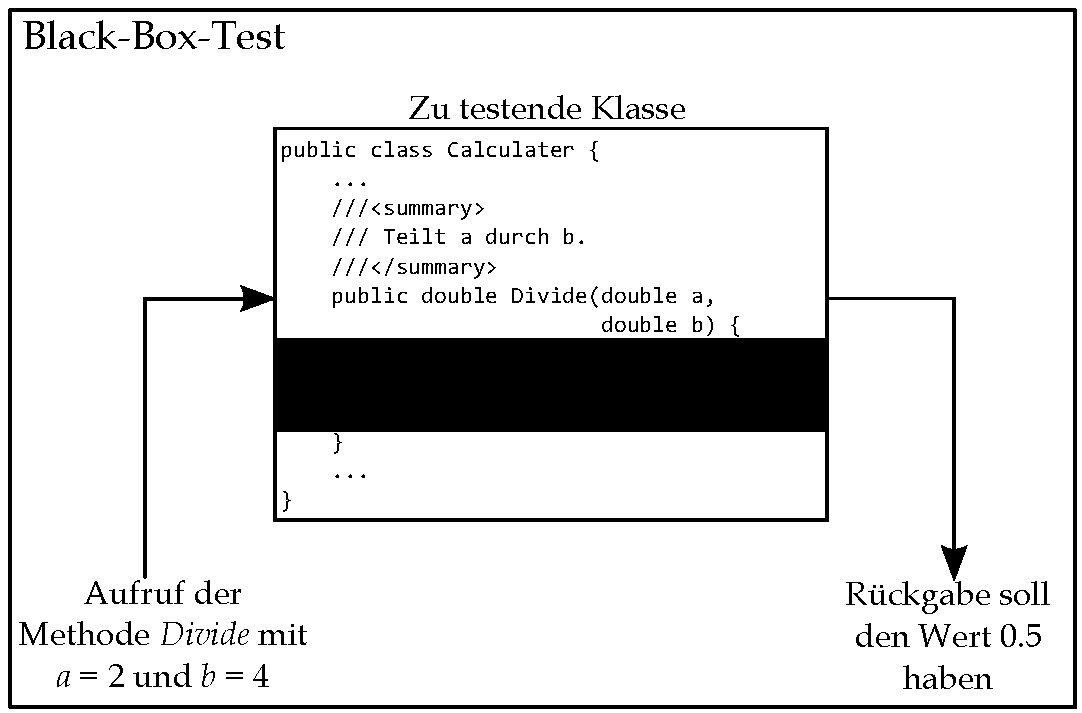
\includegraphics[width=0.8\linewidth]{./images/Kapitel_Einleitung/Black_Box_Test.pdf}
\caption[Schematische Darstellung eines Black-Box-Tests]{Schematische Darstellung eines Black-Box-Tests\\Öffentliche Klassen und Methoden, sowie deren Beschreibungen sind dem Entwickler bekannt. Die konkrete Implementierung allerdings ist nicht einsehbar. Der Test verifiziert das Verhalten der zu testenden Klasse.}
\label{fig:Black_Box_Test}
\end{figure}

\clearpage

\paragraph{Akzeptanztests} sollen die Korrektheit des Verhaltens eines ganzen Systems prüfen. Dabei soll er sowohl die Benutzerschnittstelle, als auch die einzelnen Komponenten und die Systemressourcen abdecken. Allerdings testen diese nicht die innere Struktur des Systems (sind also Black-Box-Tests), sondern sollen gewährleisten, dass ein System sich so verhält, wie es der Kunde im Lastenheft definiert hat. Idealerweise verwendet der Test dabei nur die Schnittstellen, die ein Kunde auch verwenden würde (z.B. über Eingaben auf der GUI), um möglichst nahe an ein natürliches Verhalten zu kommen.\\
Akzeptanztests können durchaus länger dauern, da sie das gesamte Verhalten eines Systems repräsentieren, welches nur nach größeren Veränderungen getestet werden muss.

\begin{figure}[h]
\centering
	\begin{subfigure}[b]{0.29\textwidth}
	\centering
	\captionsetup{justification=centering}
	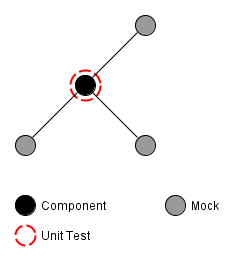
\includegraphics[width=\textwidth]{./images/Kapitel_Einleitung/Unit_Test.png}
	\caption{Unit-Test}
	\label{fig:Unit_Test}
	\end{subfigure}
	\begin{subfigure}[b]{0.29\textwidth}
	\centering
	\captionsetup{justification=centering}
	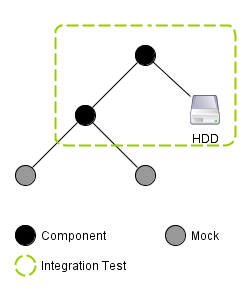
\includegraphics[width=\textwidth]{./images/Kapitel_Einleitung/Integrations_Test.png}
	\caption{Integrationstest}
	\label{fig:Integration_Test}
	\end{subfigure}
	\begin{subfigure}[b]{0.39\textwidth}
	\centering
	\captionsetup{justification=centering}
	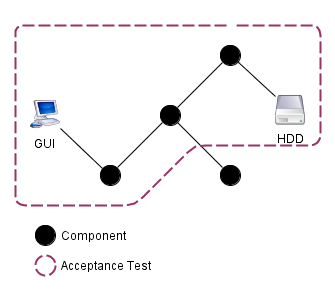
\includegraphics[width=\textwidth]{./images/Kapitel_Einleitung/Akzeptanz_Test.png}
	\caption{Akzeptanztest}
	\label{fig:Acceptance_Test}
	\end{subfigure}
\caption[Schematische Darstellung der unterschiedlichen Testarten]{Schematische Darstellung der unterschiedlichen Testarten\\(a) testet die einzelnen Methoden einer Komponente. Alle anderen benötigten Komponenten sollten als Mock-Objekte eingebunden werden.\\(b) testet das Verhalten mehrere Komponenten und eventuell im Zusammenhang mit Systemressourcen\\(c) testet einen Großteil der Komponenten eines Programms mit den Systemressourcen nach den Anforderungen des Kunden.\\
Quelle: \url{http://schneide.wordpress.com/2011/09/05/a-shot-at-definitions-beyond-unit-test/}}
\label{fig:UnitIntegrationAcceptanceTest_Comparison}
\end{figure}
\clearpage

\subsection{Grundsätze und Funktionsweise von TDD}

Die testgetriebene Entwicklung arbeitet nach dem an und für sich einfachen Prinzip, die Tests \textbf{vor} dem Produktivcode zu schreiben. Um TDD richtig anzuwenden, sollten ein paar Dinge beachtet werden. Dennoch überwiegen die daraus resultierenden Vorteile diesen Mehraufwand. In diesem Abschnitt erläutern wir welche das sind, wie der Ablauf von TDD ist und was es dabei zu beachten gilt. Dabei orientieren wir uns an dem Buch \textit{Growing Object-Oriented Software, Guided by Tests} \cite{FRE10}.

Bei der testgetriebenen Entwicklung schreibt man zunächst einen Unit-Test, der das Verhalten der zu testenden Komponente definiert. Da deren innere Struktur unbekannt ist, wird dieser automatisch als ein Black-Box-Test implementiert. Dieser muss anfangs fehlschlagen, da die Komponente noch nicht implementiert, beziehungsweise nicht vorhanden ist. Danach sollte man diese auf möglichst einfache Art und Weise implementieren, damit der Test erfolgreich ausgeführt wird. Dadurch vermeidet man überflüssigen Code. Anschließend sollte der Test erweitert werden um die Kontrolle über potentielle Fehler zu behalten (White-Box-Test). Das Resultat hat Eigenschaften beider Testarten und wird deswegen auch als \textit{Grey-Box-Test}\footnote{\url{http://de.wikipedia.org/wiki/Grey-Box-Test}} bezeichnet. Abschließend refactored man seinen Produktivcode, falls dies nötig sein sollte. Wann und wie man refactoren sollte wird später angesprochen. Für detailliertere Informationen verweisen wir auf \cite{FOW99}.\\
Dieser Vorgang wird solange wiederholt, bis alle benötigten Komponenten und Funktionen implementiert sind. Diesen Zyklus kann man mit identischen Zyklen für Integrations- und Akzeptanztests umschließt, sodass eine größere und realitätsnähere Testabdeckung entsteht.

Ein großer Vorteil von TDD ist, dass man automatisch jede Komponente mit Tests überwacht. Dies ist nicht der Fall, wenn man die Tests nach dem Produktivcode schreiben würde. Das liegt daran, dass die Tests meistens gegen Ende der Entwicklung geschrieben werden. Zu diesem Zeitpunkt ist der Druck auf die Entwickler allerdings am größten, weswegen im Zweifelsfall auf Tests verzichtet wird, da diese keine weiteren Funktionalitäten hervorbringen. Außerdem könnten die Komponenten zu einem so späten Zeitpunkt sehr stark miteinander verbunden sein, wodurch die einzelnen Tests groß und unübersichtlich werden. Sollten trotz alldem Tests entwickelt werden, müssen alle Funktionalitäten auf einmal getestet werden, was eine undankbare Aufgabe darstellt. TDD hat hier den Vorteil, dass Tests und Produktivcode abwechselnd Stück für Stück implementiert werden.\\
Ein weiterer positiver Aspekt von TDD ist, dass die Entwickler wesentlich schneller und öfter Feedback über ihr Programm erhalten. Dies ermöglicht einem die Qualität seines Produkts erheblich zu steigern, da man auf Fehler und Unstimmigkeiten mit den Kundenwünschen aufmerksam gemacht wird. Dies ist bei Spielen besonders wichtig, da es mit der Kundenzufriedenheit steht und fällt (besonders wenn man noch keine große Fangemeinde etablieren konnte).\\
TDD ermöglicht es einem, leichter wartbare und erweiterbare Systeme zu schreiben. Denn dadurch, dass die Funktionen eine nach der anderen implementiert werden, ist es modularer und es entstehen weniger Abhängigkeiten zwischen den einzelnen Komponenten (vor allem, wenn man konsequent Mock-Objekte verwendet). Wenn man zusätzlich noch viele Interfaces einsetzt, können neue Funktionalitäten leichter nachträglich hinzugefügt werden. Durch die breite Testabdeckung ist das System zudem robuster gegenüber Fehler durch Änderungen, wodurch man leichter refactoren und sorgenfreier entwickeln kann, da daraus resultierende Defekte sofort erkannt werden.\\
Dadurch, dass die Tests geschrieben werden ohne dass man Kenntnis darüber hat wie die innere Struktur aussieht, entsteht besser lesbarer Code. Man hat nur die Vorgabe was der Zweck der aktuellen Komponente sein soll und kann die Methoden entsprechend benennen. Es hilft einem auch, zu entscheiden, welche Methoden von außen sichtbar sein sollen und welche nur der konkreten Implementierung bekannt sein müssen. Dadurch erhält man wesentlich schlankere und übersichtlichere Schnittstellen.\\
Ließen sich diese Vorteile für die Spielentwicklung einsetzen, würde dies einen erheblichen Fortschritt darstellen.

Um die oben aufgeführten Vorteile zu erhalten, sollte - außer dass man die Tests vor dem Produktivcode schreibt - noch einiges beachtet werden. Steve Freeman und Nat Pryce haben in \cite[Seite 6]{FRE10} eine goldene Regel des TDD aufgestellt:

\begin{quotation}
\textbf{\textit{\grqq Never write new functionality without a failing test.\grqq}}
\end{quotation}

Dies soll verhindern, dass der TDD-Zyklus nicht unterbrochen wird und dadurch manche Codeabschnitte ungetestet bleiben. Außerdem hilft es einem keine unnötigen Funktionen einzubauen, die vom Kunden nicht gewünscht sind. Denn die Tests orientieren sich an den Vorgaben des Kunden und solange man die Tests immer zuerst schreibt, wird auch nur diese Funktionalität entwickelt.\\
Als äußerst wichtig werden auch Akzeptanztests angesehen, die das Verhalten eines realen Anwenders möglichst genau simulieren. Sie sollen nur über die definierten Schnittstellen mit dem System kommunizieren, ohne die interne Implementierung direkt aufzurufen. Solche Tests bezeichnen sie als \textit{End-To-End-Tests} und sollen das System so testen, wie es an den Kunden ausgeliefert werden soll. Dazu gehört, dass die Unit-Tests durchlaufen werden, die benötigten Pakete eingebunden werden, das System in einer produktiv-ähnlichen Umgebung gebaut wird und die Akzeptanztests ausgeführt werden. Diese Art des Testens stellt einen erheblichen Aufwand dar, allerdings kann man erst dadurch sagen, dass das System auch beim Kunden fehlerfrei funktioniert.

Bevor man mit der testgetriebenen Entwicklung produktiv werden kann, muss man ein Grundgerüst für das Projekt bauen. Dieses wird als \textit{laufendes Skelette} \cite[orig. \textit{walking Skeleton}, Seite 32]{FRE10} bezeichnet und stellt die kleinste mögliche Implementierung einer Funktionalität dar, welche sich automatisch bauen lässt und worüber man einen End-To-End-Test schreiben kann \cite{COC04}. Für das Grundgerüst benötigt man einen kleinen Erstentwurf der Programmstruktur. Dieser soll noch keine konkreten Methoden oder Attribute enthalten, sondern nur darstellen welche Komponenten voraussichtlich gebraucht werden und wie diese miteinander kommunizieren. Hierbei orientiert man sich am besten an den Kundenanforderungen.\\
Dadurch, dass zu Beginn die konkrete Struktur unklar ist, ist das Schreiben von Tests am Anfang aufwendiger und chaotisch. Des weiteren kann es zu vielen nachträglichen Änderungen kommen, da man während der Entwicklung neue Erkenntnisse gewinnt. Allerdings ist das Ende des Projekts wesentlich kontrollierter, da man bereits eine solide Testbasis hat, welche einem Gewissheit gibt, dass das System so funktioniert wie es soll. Schreibt man die Tests am Ende, hat man das Problem sowohl diese, als auch die auf der Strecke gebliebenen Funktionen zu implementieren. Die testgetriebene Entwicklung verlagert den stressigen Teil des Projekts an den Anfang, wobei man zu diesem Zeitpunkt besser auf die auftretenden Probleme eingehen kann, anstatt kurze Zeit vor dem Veröffentlichungstermin.

Um den Zyklus der testgetriebenen Entwicklung am Laufen zu halten, gilt es weitere Dinge zu beachten, welche in \cite{FRE10} ab Seite 39 ausführlich beschrieben werden. Die wichtigsten Verhaltensregeln stellen wir hier nun kurz vor:

\begin{description}
\item[\small Jede neue Funktionalität soll mit einem Black-Box-Test beginnen]~\\
	Dadurch definiert man das Verhalten, ohne die innere Struktur zu berücksichtigen und erhält schlanke Schnittstellen. Die konkrete Implementierung kann sich nun laufend ändern und man hat dennoch einen Test der sicherstellt, dass das Verhalten korrekt ist.
\item[\small Unterscheiden zwischen fortschrittsmessenden und Rückschritt erkennenenden Tests]
	Neue Akzeptanztests stellen eine noch nicht implementierte Funktion dar. Sobald sie fehlerfrei ausgeführt werden, ist die Funktion fertig. Sie messen demnach den Fortschritt des Projekts.\\
	Sobald ein Akzeptanztest implementiert wurd,e misst er keinen Fortschritt mehr, sondern stellt sicher dass die Funktion fehlerfrei bleibt. Schlägt ein Test fehl, hat er einen Rückschritt erkannt.
\item[\small Tests sollen wohlformuliert sein]~\\
	Die Tests sollen das Verhalten, welches sie testen, möglichst genau beschreiben, sodass man auch bei späterem Betrachten weiß, was getestet wird. Schlägt der Test fehl, sollte eine aussagekräftige Fehlermeldung ausgegeben werden.
\item[\small Tests zuerst fehlschlagen lassen]~\\
	Nachdem man einen Test geschrieben hat, soll man diesen immer zuerst fehlschlagen lassen, bevor man den Produktivcode dazu schreibt. Dadurch erkennt man, ob einen die Fehlermeldung an die richtige Stelle leitet. Dadurch lässt sich ein später auftretender Fehler leichter beheben. Außerdem erkennt man Design-Fehler, falls der Test in einer anderen Weise als erwartet fehlschlägt.
\item[\small Teste das Verhalten, nicht die Methoden]~\\
	Es ist wichtiger ein korrektes Verhalten zu testen und nicht die einzelnen Zeilen jeder Methode. Auch eine hundertprozentige Testabdeckung garantiert kein fehlerfreies System. Tests sollten so formuliert werden, dass sie aussagen was sie testen und nicht welche Methode.
\item[\small Man soll auf seine Tests hören]~\\
	Wenn man auf eine schwierig zu testende Stelle trifft, sollte man sich nicht fragen, wie man diese testen kann, sondern warum es schwer ist sie zu testen. Dies ist meistens ein Anzeichen dafür, dass die Struktur refactored werden muss. Denn wenn etwas schwierig zu testen ist, ist es meist auch schwer zu ändern oder zu erweitern. Dies fällt allerdings meist erst später auf, weswegen man das Problem lösen sollte, solange es noch \grqq frisch\grqq~ist.
\end{description}

Da Refactoring ein wesentlicher Bestandteil der testgetriebenen Entwicklung ist, steht in \cite{FRE10} wann man refactoren sollte und wie man am besten mit den Tests verfährt. Wichtig ist, dass Refactoring keinen Geschwindigkeits- oder Funktionsvorteil bringt, sondern nur besser Wartbarkeit und Lesbarkeit. Die Hinweise beziehen sich meist darauf, dass nur die benötigten Teile einer Komponente nach außen sichtbar sein sollen und der Rest geheim bleibt. Außerdem helfen sie die einzelnen Komponenten richtig zu strukturieren, indem große gespalten werden und häufig auftretende Gruppen von Merkmalen zu einer neuen Komponente zusammengefasst werden. Auch hier wollen wir die wichtigsten Tipps vorstellen:

\begin{description}
\item[\small Teilen großer Komponenten]~\\
	Wenn eine Komponente während der Entwicklung sehr groß wird, kann man sie meistens in kleinere Komponenten unterteilen, welche anschließend separat getestet werden. Dadurch erhält man eine modulare Struktur und kleinere, übersichtlichere Tests. Außerdem werden einem die Abhängigkeiten seines Programms vor Augen geführt.
\item[\small Definieren eines neuen Services]~\\
	Wenn man den einzelnen Komponenten immer weitere Verhalten zuweist, kann es sein, dass diese nicht in die Komponente gehören. In diesem Fall sollten die Verhalten in einen neuen Service ausgelagert werden.\\
	Dafür wird dieser zunächst (zum Beispiel in Form eines Interfaces) definiert und im Unit-Test der Komponente gemocked. Anschließend werden Tests für diese Komponenten geschrieben.
\item[\small Bündelung von Komponenten]~\\
	Falls man eine Menge zusammenhängender Komponenten findet, kann man diese zu einer neuen Komponente vereinen. Diese verringert die Komplexität, da nur die relevanten Teile nach außen sichtbar sind. Dadurch wird die Domain besser verständlich und die Tests werden übersichtlicher, da man die neue Komponente separat testen kann.
\end{description}

Hält man sich an alle genannten Verhaltensregeln, bekommt man ein leichter wartbares und verständliches System mit den oben aufgeführten Vorteilen. Allerdings muss man sich an die Art der testgetriebenen Entwicklung erst gewöhnen, sollte diszipliniert sein und seine Erfahrung damit machen, bevor man damit souverän entwickeln kann.
\pagebreak

\section{Unity 3D}

\textit{Unity 3D} (mittlerweile nur noch \textit{Unity}) ist eine Spiele-Engine, welche für viele verschiedene Anwendungen, wie Spiele, Lernsoftware, sowie 3D-Animationsfilme verwendet wird. Der Hersteller bezeichnet die Software selber als \textit{Spieleentwicklungs-Ökosystem}\footnote{Zu lesen unter \url{http://unity3d.com/unity/}}, da sie neben der Engine selber eine komplette Entwicklungsumgebung für Spiele bietet.\\
Die Umgebung erlaubt es einem, die Spiele auch auf andere Plattformen zu portieren, wie zum Beispiel für Android auf Smartphones oder für Webanwendungen. Dies macht die Engine sehr flexibel und ist auch ein Grund für die weite Verbreitung. Der Spielecode für das Spiel lässt sich in verschiedenen Sprachen programmieren, die beim Übersetzen alle von der Unity-Umgebung in die Common Intermediate Language überführt werden, eine Assemblersprache, die erst beim Ausführen in einer Laufzeitumgebung (.NET oder Mono) in nativen Maschinencode übersetzt wird. Die verfügbaren Scriptsprachen sind JavaScript, C\# und Boo\footnote{Weitere Infos zu Boo unter \url{http://boo.codehaus.org/}}.


\paragraph{Unity als Entwicklungsumgebung} Im Mittelpunkt steht ein Szeneneditor, der es ermöglicht die einzelnen Spielszenen zu gestalten, indem die Spielelemente in einem 3D-Editor so angeordnet werden, wie sie im späteren Spiel zu sehen sind. 
Ein Element in einer Szene wird dabei \textit{GameObject} genannt, die Elemente, die zum Einbau bereit stehen, nennt man \textit{Assets}. Ein \textit{Asset} kann dabei vieles sein: Zum Beispiel 3D-Models (\textit{Meshes}), Skripte, Texturen oder Audio-Dateien. \textit{GameObjects} lassen sich beliebig hierarchisch anordnen, um sie so zu gruppieren, oder logisch zu strukturieren. So kann zum Beispiel ein \textit{GameObject} \textit{Spielfigur} die einzelnen Körperteile als Unterobjekte haben, wenn sie als eigene Objekte behandelt werden sollen. Dies vereinfacht zusätzlich den späteren Zugriff auf diese Objekte.\\
Jedem \textit{GameObject} können sogenannte \textit{Components} zugeordnet werden, welche die Eigenschaften und das Verhalten dieses Objektes beschreiben. So muss immer ein \textit{Transform}-Komponente vorhanden sein, das die Position in der Welt, sowie die Rotation und die Skalierung beschreibt. Komponenten können auch Skripte sein, die bei jedem Frame für dieses \textit{GameObject} ausgeführt werden. Es gibt auch Komponenten, die ein \textit{GameObject} zu einem physikalischen Objekt machen, zum Beispiel um ihm eine Gravitationskraft zu geben, oder um Kollisionen zu erkennen. Der Mechanismus zur Kollisionserkennung ist mit Events implementiert. Das heißt, dass in den Skripten eines \textit{GameObjects} zum Beispiel eine \textit{OnCollisionEnter}-Methode vorhanden sein kann, die aufgerufen wird, wenn es mit einem anderen \textit{GameObject} kollidiert. Dies muss nicht unbedingt heißen, dass zwei 3D-Models in der Spielwelt aufeinandertreffen, wenn zum Beispiel ein Projektil einen Gegner trifft. Man kann auch spezielle Kollisions-Boxen für ein Objekt bestimmen, damit zum Beispiel erkannt wird, wenn ein \textit{GameObject} in einen bestimmten Bereich der Spielwelt kommt. Komponenten können auch Texturen, 3D-Modelle, oder Geräuschquellen sein.\\
3D-Modelle können theoretisch auch in einem eigenen 3D-Modellierungstool bearbeitet werden, dies ist allerdings noch nicht ausgereift und wenig komfortabel. Für diese Aufgabe gibt es auch bessere Tools, wie zum Beispiel Blender, welches auch kostenlos verfügbar ist.\\
Mit integriert in die Unity-Umgebung ist Mono-Develop, eine alternative Entwicklungsumgebung für .NET-Sprachen, welche man direkt aus Unity aufrufen kann. Unity bietet die Möglichkeit, das Spiel direkt aus dem Editor übersetzen zu lassen. Dies kann mit einem richtig Build geschehen, allerdings auch für Testzwecke direkt im Editor. Dabei wird aus dem 3D-Viewport einfach die Spieleansicht. Das eignet sich gut für ein schnelles Ausprobieren der Szene, ist allerdings durch eine auf Debugging ausgelegte Kompilierung nicht so schnell, wie der endgültige Build. Am Ende sind die Skripte in einer eigenen .NET-Programmbibliothek vorkompiliert und werden so von der Engine eingebunden.

\paragraph{Unity als Engine} Unity bietet als Spiele-Engine verschiedene Mechanismen, die man bei einem Spiel benötigt. Dies ist in erster Linie eine Grafik-Engine, die die gegebenen Modelle und Texturen in ein Bild auf dem Bildschirm verwandelt. Dazu kommen Engines, die Physikberechnungen durchführen, Audio abspielen, sowie Netzwerkverbindungen für Multiplayer-Spiele bieten.\\
Diese ganzen Engines bilden den Rahmen um das entwickelte Spiel, also die eigenen Skripte, bzw. sonstige eigene Logik. Man muss keine eigene Hauptschleife entwickeln, denn Unity bindet die Skripte ein und führt diese zu entsprechenden Zeitpunkte aus. In jedem Spiel gibt es eine Hauptschleife, die für jeden Frame, der auf dem Monitor angezeigt wird, ausgeführt wird und die Berechnungen durchführt. Dazu wird bei jedem Durchlauf der aktuelle Zustand, sowie Eingaben, wie zum Beispiel Tastendrücke, registriert und daraus der Folgezustand berechnet und auf dem Monitor ausgegeben. Diese Hauptschleife bildet den Kern jedes Spiels.\\
Die Skripte, die nun programmiert werden und das Verhalten der einzelnen Elemente im Spiel beschreiben, müssen von der Unity-Engine interpretierbar sein. Dafür können verschiedene Methoden implementiert werden. \\
Für die folgenden Codebeispiel wurde C\# als Skriptingsprache gewählt, da sie auch unsere verwendete Sprache bei der Entwicklung des Prototypen ist, was später detaillierter betrachtet wird. Bei C\# (und auch bei Boo) gibt es eine Besonderheit, die bei JavaScript nicht beachtet werden muss. Jede Skriptklasse muss hier von \textit{MonoBehaviour} erben. Damit deklariert man diese Klasse als Skript eines \textit{GameObjects} und wird automatisch bei der Engine registriert.\\
Die wichtigste Methode ist \textit{Update()}, welche von der Engine bei jedem Frame aufgerufen wird. Hier müssen alle notwendigen Berechnungen für dieses Objekt und die Änderungen der Spielwelt ausgeführt werden.
Ein sehr einfaches Beispiel für ein Objekt, das sich um die y-Achse drehen soll sieht wie folgt aus.\\

\begin{lstlisting}[caption={[Einfache Skript-Klasse mit Update-Methode]Einfache Skript-Klasse mit Update-Methode}]
using UnityEngine;

public class Beispiel : MonoBehaviour{
	void Update(){
		transform.Rotate(0,5,0);
	}
}
\end{lstlisting}

Die Membervariable \textit{transform} wird von \textit{MonoBehaviour} geerbt und ist eine Referenz auf die zwingend vorhandene \textit{Transform}-Komponente. Diese Komponente lässt sich über verschiedene Methoden beeinflussen, womit man das Objekt drehen, verschieben, oder skalieren kann.\\
Wie man in diesem Beispiel sieht, wird das Objekt bei jedem Frame um den gleichen Winkel gedreht. Dies würde mit einer gleichbleibenden Framerate funktionieren, allerdings kommt das in der Praxis nicht vor. Dafür gibt es in der Engine einen Zeitmechanismus, die Klasse \textit{Time}, die einem Zugriff auf unterschiedliche Zeitinformationen liefert. Dazu gehört \textit{deltaTime}, welche die Zeit in Sekunden beinhaltet, die die Berechnung des letzten Frames gebraucht hat. Damit lässt sich die Methode von oben folgendermaßen schreiben.
\pagebreak

\begin{lstlisting}[caption={[Einfache Update-Methode mit deltaTime]Einfache Update-Methode mit deltaTime}]
	void Update(){
		transform.Rotate(0,5*Time.deltaTime,0);
	}
\end{lstlisting}

Hiermit wird das Objekt nur um 5 Einheiten pro Sekunde verschoben, was die Berechnung unabhängig von der Framerate macht.

Eine weitere wichtige Methode ist \textit{OnGUI()}, in der Dinge implementiert werden, die in der GUI ablaufen sollen. Als GUI bezeichnet man in einem Spiel die Ebene, die über der 3D-Darstellung liegt, wo Menüs, Lebensanzeigen, oder auch Munitions-Stände oder sonstige Status-Elemente platziert werden. \textit{OnGUI} wird bei jedem GUI-Event aufgerufen, wenn zum Beispiel auf ein GUI-Element geklickt wird. Dies kann auch häufiger als der Aufruf von \textit{Update} stattfinden, weshalb diese Aktionen in \textit{OnGUI} verarbeitet werden müssen.

Ein weitere Methode ist \textit{OnCollisionEnter(Collision c)}, welche in einem \textit{GameObject}-Skript aufgerufen wird, wenn ein anderes Objekt in den Kollisionsbereich eintritt. Damit dieser Event-Handler aufgerufen wird, müssen beide Spielobjekte eine sogenannte \textit{Rigidbody}-Komponente haben, welche physikalische Eigenschaften für das Objekt festlegt. Der Methode wird beim Aufruf ein \textit{Collision}-Objekt übergeben, in dem die Daten des kollidierenden Objektes stehen.
\pagebreak

\section{Entwicklungsumgebung}

Wie oben beschrieben, bietet die Unity SDK die Möglichkeit mit mehreren Programmiersprachen zu entwickeln. Um alle Möglichkeiten der objektorientierten Entwicklung nutzen zu können, haben wir uns dazu entschieden den Prototypen in C\# zu schreiben. Dementsprechend nutzen wir neben der Unity SDK noch \textit{Visual Studio 2012} zum programmieren der Logik. Um effizienter entwickeln zu können und aufgrund der besseren Refactoring-Möglichkeiten haben wir \textit{Resharper}\footnote{Für nähere Informationen zu Resharper siehe \url{http://www.jetbrains.com/resharper/}.} installiert. Zusätzlich dazu bietet es einen wesentlich übersichtlicheren Test-Explorer, wie man in der Abbildung auf der nächsten Seite sehen kann.

Zur Verteilung der Aufgaben haben wir Bugzilla\footnote{Für nähere Informationen zu Bugzilla siehe \url{http://www.bugzilla.org/about/}} verwendet. Um die Bugs zu editieren und übersichtlich darzustellen wurde die Lite Version von Deskzilla genutzt.

Damit wir parallel an dem Prototypen arbeiten können, musste das Projekt in einem Git-Repository gespeichert werden, wobei man beim Aufsetzen des Repositories einiges beachten sollte, damit die Verwaltung auch funktioniert. Dies liegt daran, dass manche Dateien in einem Unity-Projekt nur relevant für die SDK des aktuellen Benutzers sind und die Entwicklungsumgebung des Anderen stören würden, falls sie im Repository gespeichert werden. Andererseits befinden sich unter diesen Dateien auch benötigte Information, damit das Projekt korrekt funktioniert, wie zum Beispiel welche Skripte an einem Spielobjekt hängen. Deswegen gibt es die Möglichkeit (seit Version 3.5 auch für die kostenlose Variante von Unity) diese Informationen in Meta-Files abzuspeichern, die sich am selben Ort wie die eigentliche Dateien befinden. Danach muss man noch den Ordner \textit{Library} in das Gitignore-File aufnehmen. Sollte man mehrere Unity-Projekte in einem Repository haben, empfiehlt es sich in jedem Projektordner ein separates Ignore-File anzulegen, um nicht die vollständigen Pfade zu den \textit{Library}-Ordnern angeben zu müssen. Dadurch lassen sich die Ignore-Files für die einzelnen Projekte einfach kopieren.

Eine detaillierte Anleitung zum Verwalten eines Unity-Projekts mit externen Versionierungstools findet man unter \url{http://docs.unity3d.com/Documentation/Manual/ExternalVersionControlSystemSupport.html}.


\begin{figure}[t]
\centering
	\begin{subfigure}[b]{0.45\textwidth}
	\centering
	\captionsetup{justification=centering}
	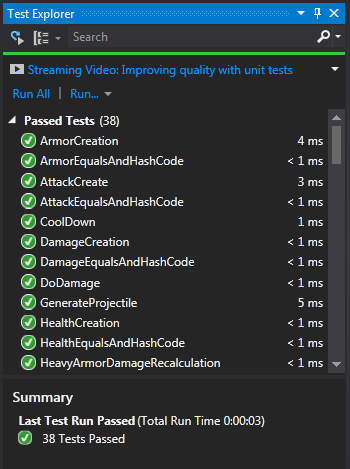
\includegraphics[width=\textwidth]{./images/Kapitel_Einleitung/VisualStudioTestExplorer}
	\caption{Visual Studio 2012}
	\label{fig:VisualStudioTestExplorer}
	\end{subfigure}
	\begin{subfigure}[b]{0.8\textwidth}
	\centering
	\captionsetup{justification=centering}
	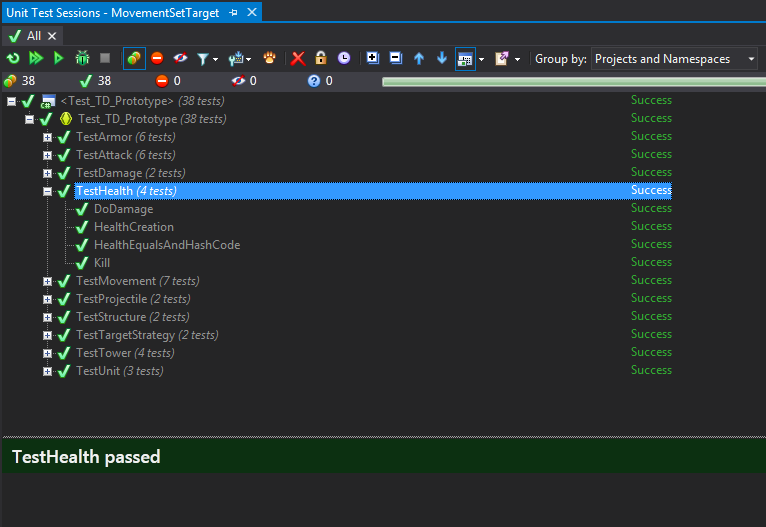
\includegraphics[width=\textwidth]{./images/Kapitel_Einleitung/ResharperTestExplorer}
	\caption{Resharper}
	\label{fig:ResharperTestExplorer}
	\end{subfigure}
\caption[Test Explorer von Visual Studio 2012 und Resharper im Vergleich]{Test Explorer von Visual Studio 2012 und Resharper im Vergleich.}
\label{fig:TestExplorerComparison}
\end{figure}
